\chapter{Object~Detection}
\label{chap:object_detection} 

\section{Introduction}

In this chapter I describe the object detector, training and evaluation metrics used in the object detection annotation system described in chapter \ref{chap:design} and used in this thesis. I describe the object detector, and describe the key differences and the motivations behind those differences in adapting this object detector for the purposes of assisting annotation.

The object detector is based off a single-shot \gls{CNN} detector called RetinaNet \cite{Lin2017}, which was selected for it's simplicity and efficiency, while having close to state of the art accuracy. Here are some of the modifications from the method in \cite{Lin2017} and brief motivation (described in more detail later in this chapter):

\begin{itemize}
    \item Shared weights between classification sub-networks. This was found to train much faster at the beginning.
    \item No normalisation of the loss function (by number of anchor matches), in order to accommodate images with no positive annotations.
    \item Training on crops of high resolution images, but evaluation on complete images.
    \item Use of cyclical learning rates in training, to accommodate incremental additions to the training set
\end{itemize}


Later in this chapter we test some of the hypotheses which led us to these decisions.

\begin{itemize}
    \item {It is possible to train object detectors at high resolution using only cropped sections; and keeping images at high resolution will provide more accurate object detection}
    \item {When training a single class object detector it will learn faster than multi-class object detectors}
    \item {When incrementally adding images through annotation; training the object detector will adapt to new examples better when using a cyclical learning rates}
\end{itemize} 

\section {Image preparation}

One thing which was noticed in the implementation of the segmentation tool from chapter \ref{chap:bootstrap} was that the original images were often much clearer than the scaled down images for a human annotator to see fine details which can be lost at lower resolution. It is not necessary to train the object detector on the same resolution as seen by a human annotator, but if a human annotator can't see important details, it would seem likely to make the task much more difficult for machine model, as well.

With that in mind I focused on preserving resolution for the annotation process. High resolution images present a cost in terms of training (and inference) time, also in terms of memory and data storage and data transfer over a network, all of which make smaller images preferable. In section \ref{sec:scale_crop} I experimentally validate this idea, comparing training with different resolutions (and crop sizes) for a selection of datasets.

The additional benefit to preserving resolution is that performance of a given object detector has generally been shown to be better with higher image resolution, when training on data with a limited number of classes, we hypothesis that it is possible to get away with larger image sizes by using smaller crops of the original images to train, as long as the objects fit in the image crops. We do some experiments on this idea in section-\ref{sec:validation}, in order to verify these assumptions.

As a counter example the images in the PASCAL VOC \cite{Everingham2008}, or COCO\cite{Lin2014} datasets have a large range of scales, distributed much more evenly with large objects occupying large portions of the image. For the majority of data experimented on in this thesis, the objects of interest occupy an area much smaller than the whole image size. An analysis of object sizes of two of the less extreme datasets compared to VOC and COCO can be seen in figure \ref{fig:box_sizes}.


\begin{figure}[ht]
\centering
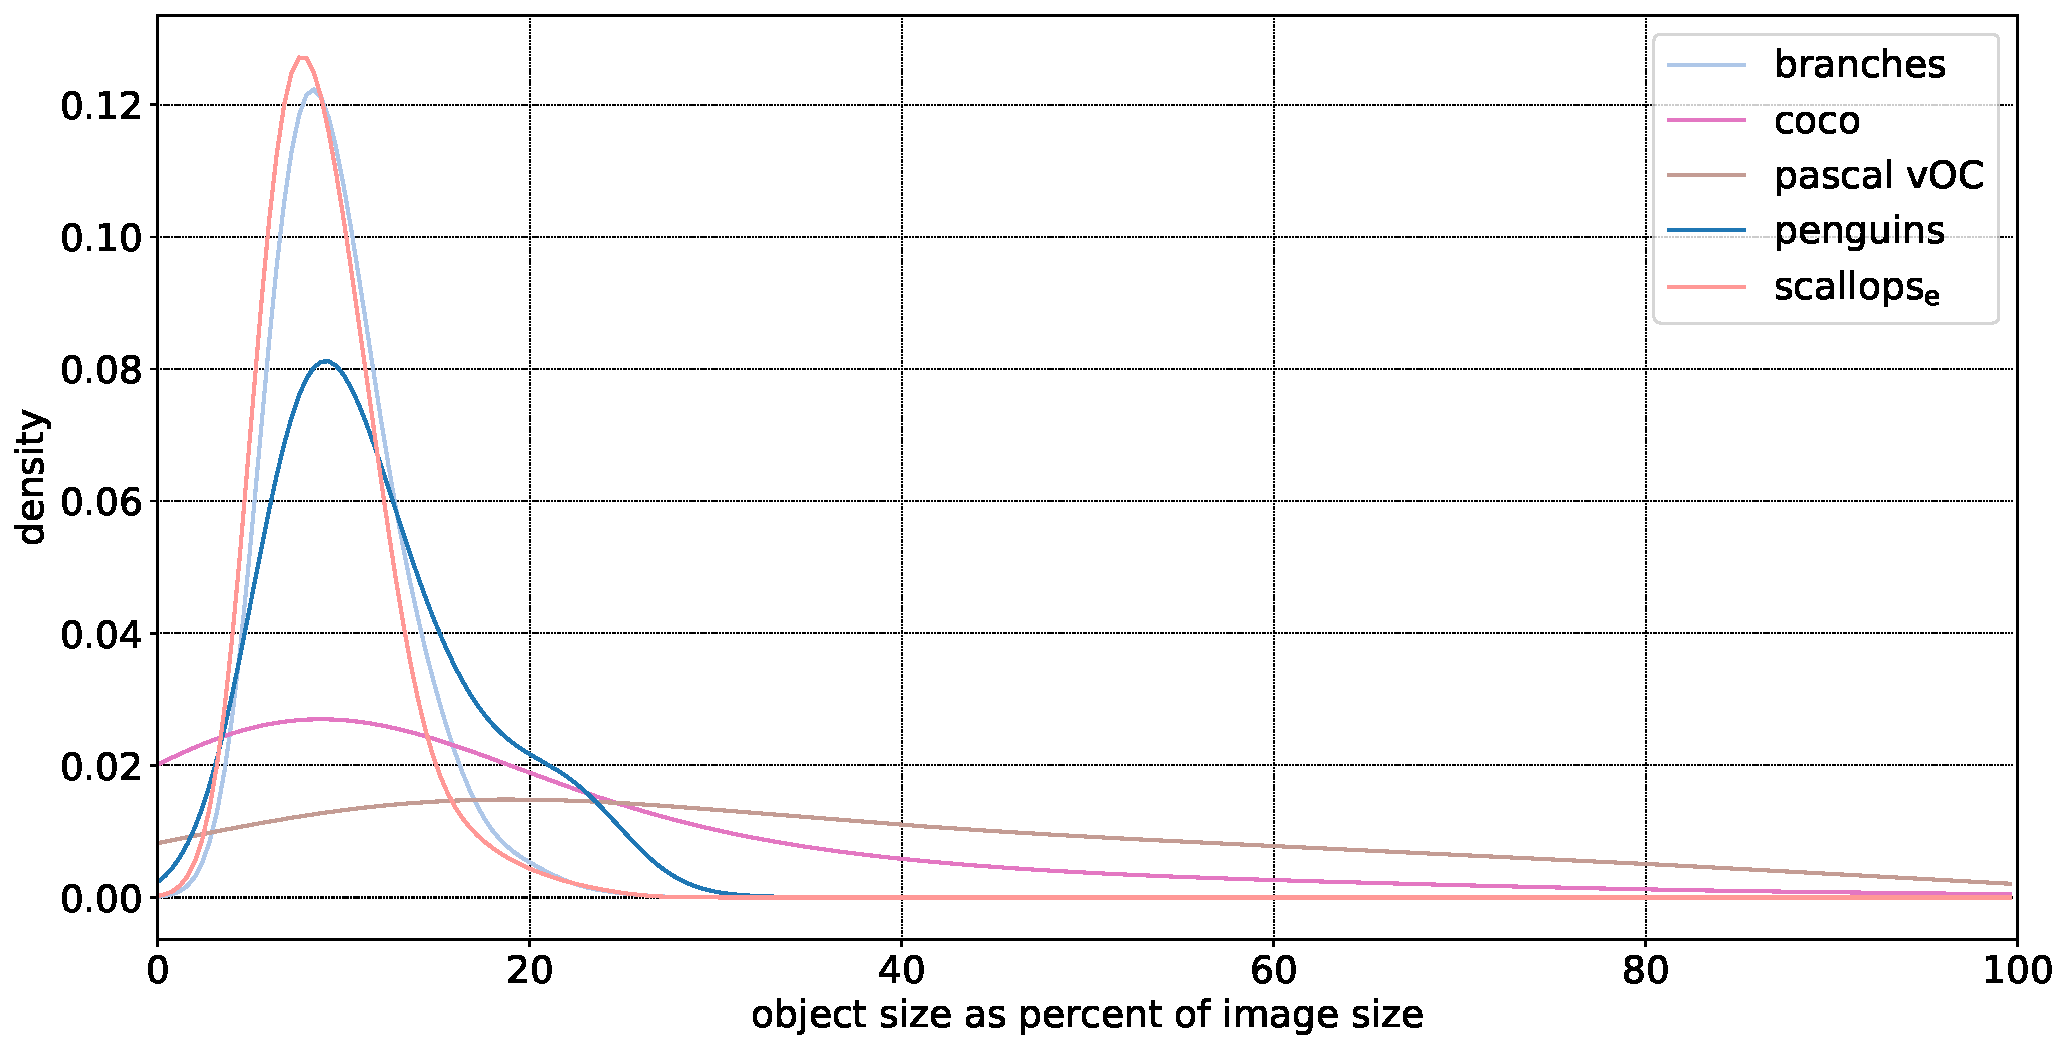
\includegraphics[width=0.9\linewidth]{charts/summaries/sizes_density.pdf}
\caption{Object bounding box size distributions as percent object to image size (average of width and height ratios) }
\label{fig:box_sizes}
\end{figure}


Use of simpler, faster models has been successful as the backbone of the object detection network (for example ResNet--18), which enables larger images in both training and evaluation. Time taken for evaluation and training is also much improved relative to using larger networks. For the smaller datasets in our experiments I did not see large improvements in accuracy when using larger backbone networks.

\begin{table}[h]
  \centering
    \caption{Ranges of parameters used for image augmentation, translation occurs as part of a cropping process}
    
  \begin{tabular}{ l  l }
    Parameter & Range \\
    \toprule
    scale (log uniform) & ${3/4}$--${4/3}$  \\ 
    aspect scale  & $ 1 \pm 0.1 $  \\ 

    brightness adjustment (additive) & $ \pm 10 $ \\ 
    contrast (multiplicative) & $ 1 \pm 0.1 $ \\ 

    gamma adjustment & $ \pm 0.1 $ \\ 

    hue shift & $ \pm 5 $ \\ 
    saturation shift & $ \pm 5 $ \\ 
    
    horizontal flips & $ P = 0.5 $ \\ 
    
    \bottomrule
  \end{tabular}
\label{fig:obj_augmentation}
\end{table}

After applying augmentation (photo-metric distortion and scaling) with parameters described in table \ref{fig:obj_augmentation} and image whitening (described below), a region is cropped from the resulting image at random. In the case where the crop region is larger than the input image, an image is created with pixels set to zero and the input image is placed at a random position within the image.

The crop sizes used in experiments, and in image annotation are specific to each dataset, ranging from $1024\times1024$ for the \emph{apples1} and \emph{apples2} datasets, down to $320\times320$ for the \emph{branches} dataset.

We employ image whitening to ensure consistency with ImageNet trained models (used as the backbone of the networks) subtracting mean (r, g, b) $ (0.485. 0.456, 0.406) $ and dividing by standard deviation $ (0.229, 0.224, 0.225) $.


\section {Object detection}

The object detection method I have been using for the following experiments is a modified RetinaNet \cite{Lin2017} as a strong near-state of the art object detector with a simple implementation. RetinaNet is a type of single shot object detector, meaning that it detects all objects together in one pass, as opposed to two stage detectors which first identify sets of bounding box proposals and then have a second pass to refine those box proposals into concrete detections. Single shot detectors (such as \gls{SSD} \cite{Liu2016a} or RetinaNet) typically achieve faster inference and training time by skipping the second refinement phase, at a slight cost of accuracy.  

Many object detection methods are based on sliding windows, where windows of fixed sizes are moved across an image and attempt to match objects of that size at each position. \gls{CNN} based object detectors achieve this using anchor boxes, where the sliding window is replaced by a simultaneous matching of boxes at each point across an image. Using a fixed set of anchor boxes limits the localisation accuracy, so the counter point to matching anchor boxes is also estimating a transformation to refine an anchor box to fit the more specific size of the object.

RetinaNet is based off Feature Pyramid Networks \cite{Lin2017a} which uses feature maps produced at multiple levels of a \gls{CNN} to classify anchor boxes of different sizes, where many smaller anchor boxes match smaller objects on higher resolution feature maps and fewer larger anchor boxes match larger objects. 

The object detection models bear close similarly to the segmentation models discussed and used in chapter \ref{chap:bootstrap}, such as UNet \cite{Ronneberger2015}. \gls{FPN} models utilise shortcut connections in the same way, the major difference from segmentation models is that anchor boxes are predicted at multiple levels, where segmentation models output mask predictions only at one resolution.


\subsection {Network architecture}
\label{sec:architecture}

Some parameters and network architectures differ from the original paper. For the most part the modifications are small things which seem to enable it to learn better on the kind of small datasets used for experiments in this work. 

These include adding extra residual layers to the decoder, shown in figure \ref{fig:detection_network}. It is more similar to the network shown in  \ref{chap:bootstrap} than the \gls{FCN} network. A key difference is that neither the weights between classification sub-networks nor box regression subnets are shared between different scales  (the original shares weights between classification sub-networks). Shared weights were found it to slow down initial training considerably in the initial phase. 

Other differences are necessary to accommodate different box sizes (usually using additional prediction outputs from earlier layers with finer anchor boxes to handle small objects).

\begin{figure}[h]
  \centering
  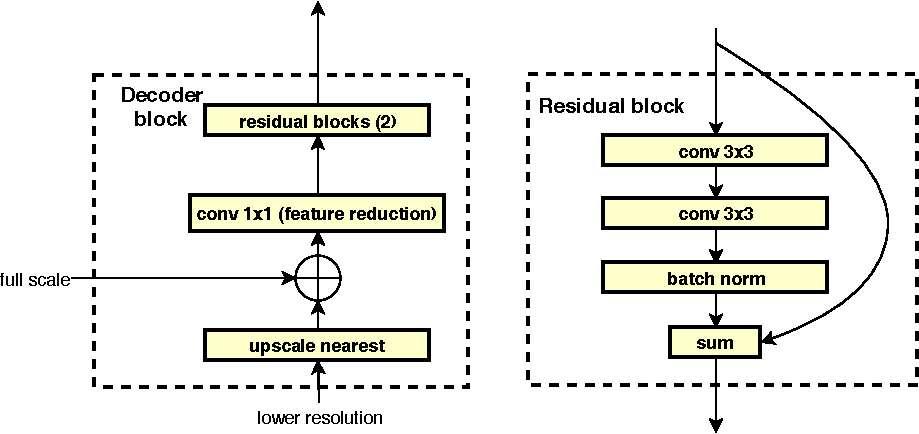
\includegraphics[width=1.0\linewidth]{figures/annotation/decoder_block.pdf}
  \caption{Decoder block, responsible for merging half resolution features with features from full resolution skip connections }  
  \label{fig:decoder_block}
\end{figure}


\begin{figure}[h]
  \centering
  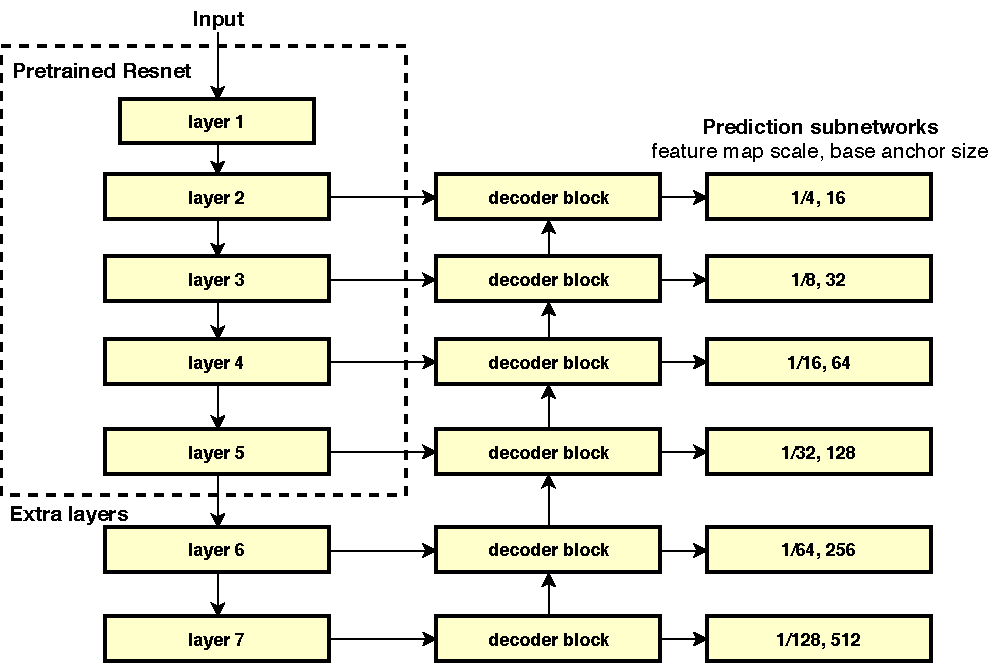
\includegraphics[width=1.0\linewidth]{figures/annotation/detection_network.pdf}
  \caption{Object detection network, built on the backbone ResNet }  
  \label{fig:detection_network}
\end{figure}

\begin{figure}
  \centering
  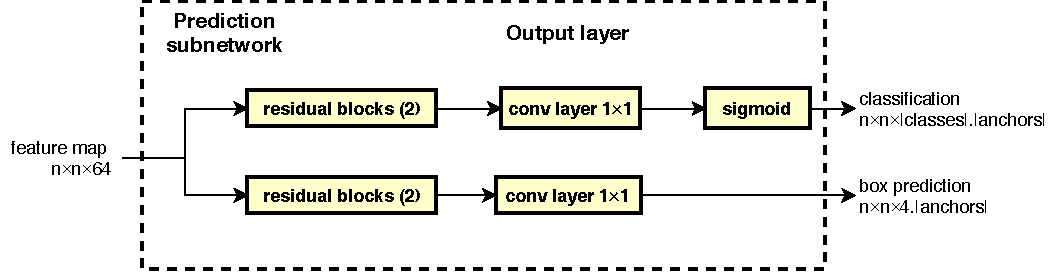
\includegraphics[width=1.0\linewidth]{figures/annotation/prediction_subnet.pdf}
  \caption{Prediction sub-network with two streams, one for classifying anchor boxes with one output per class for each anchor box, the other stream for location regression for each anchor box (shared between classes)}    
  \label{fig:prediction_subnet}  
\end{figure}




\subsection{Anchor boxes}

\begin{figure}
  \centering
  \begin{subfigure}[t]{0.33\textwidth}
  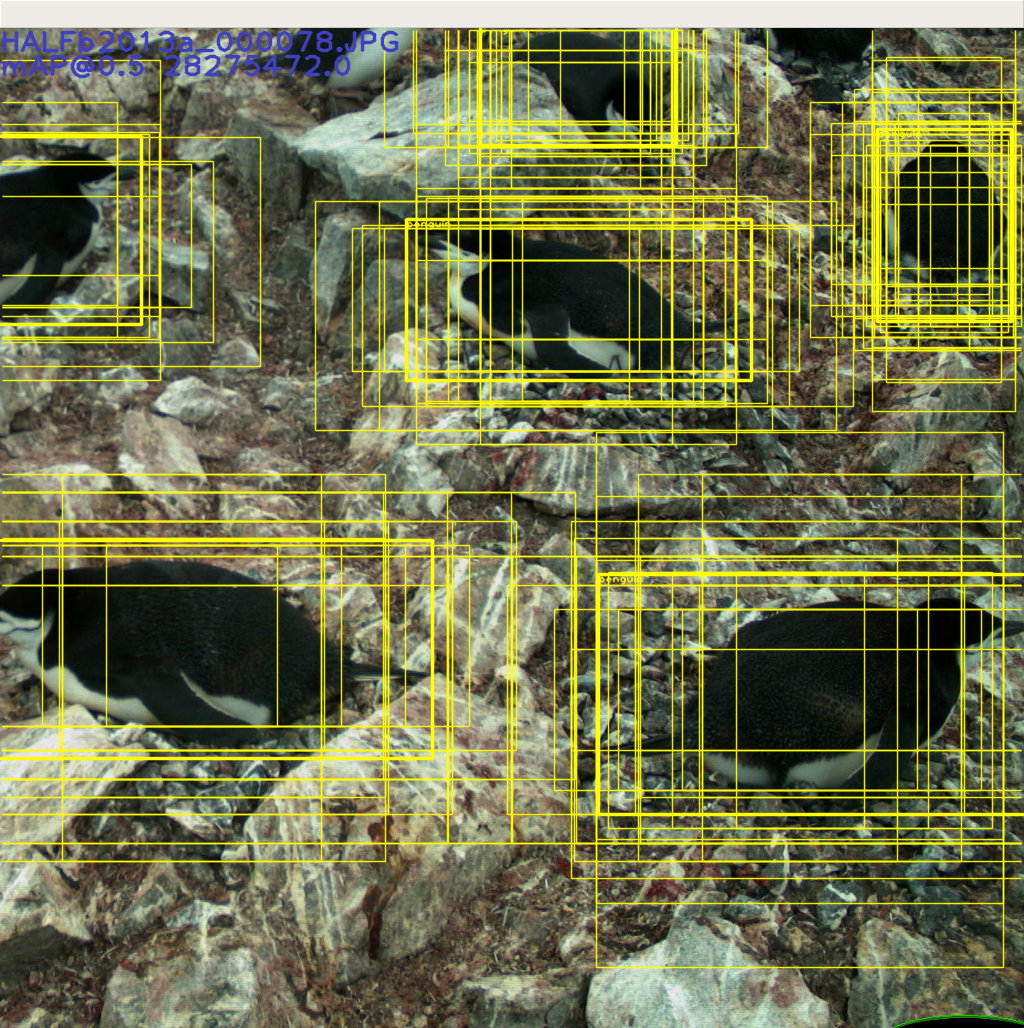
\includegraphics[width=0.95\linewidth]{figures/object/anchors.png}
  \caption{Anchor boxes from class predictions}
  \end{subfigure}%
  \begin{subfigure}[t]{0.33\textwidth}
  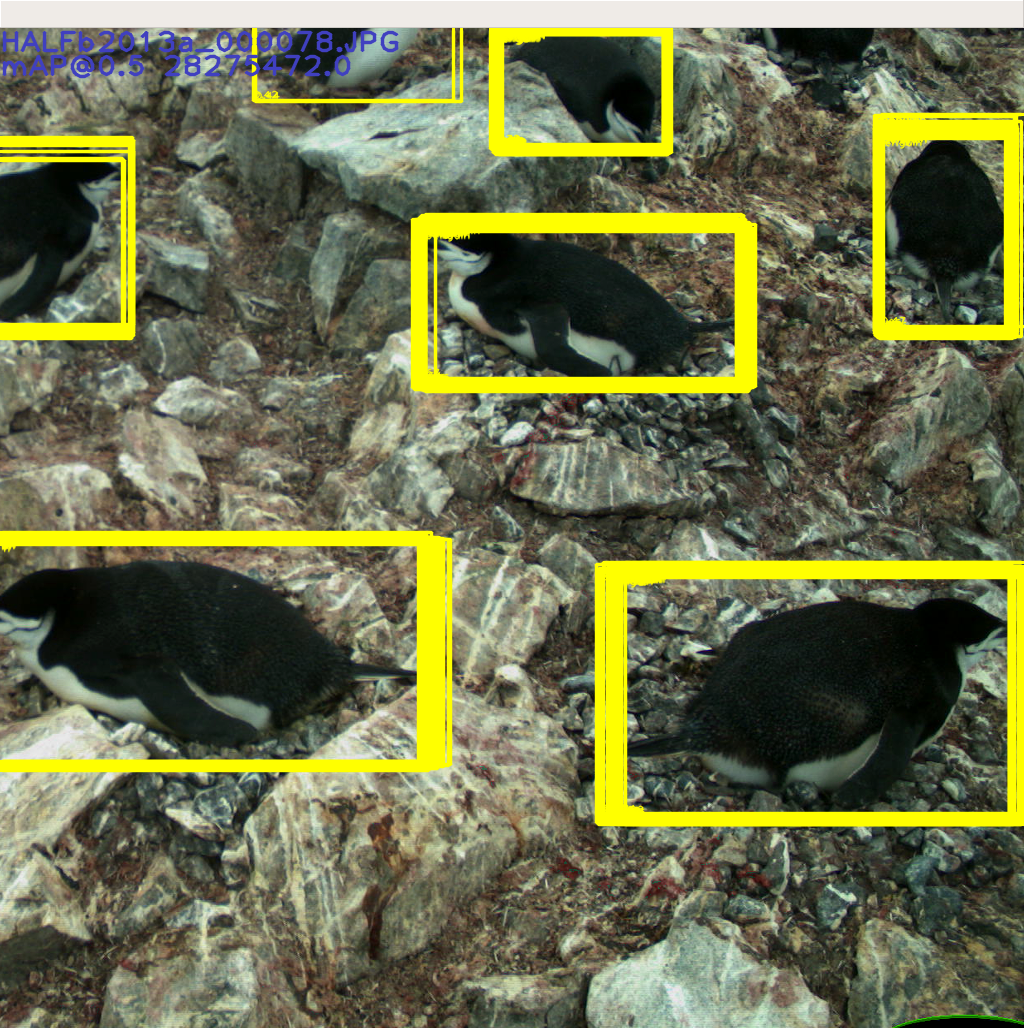
\includegraphics[width=0.95\linewidth]{figures/object/predictions.png}
  \caption{Refined anchor boxes after transformation}
  \end{subfigure}%
  \begin{subfigure}[t]{0.35\textwidth}
  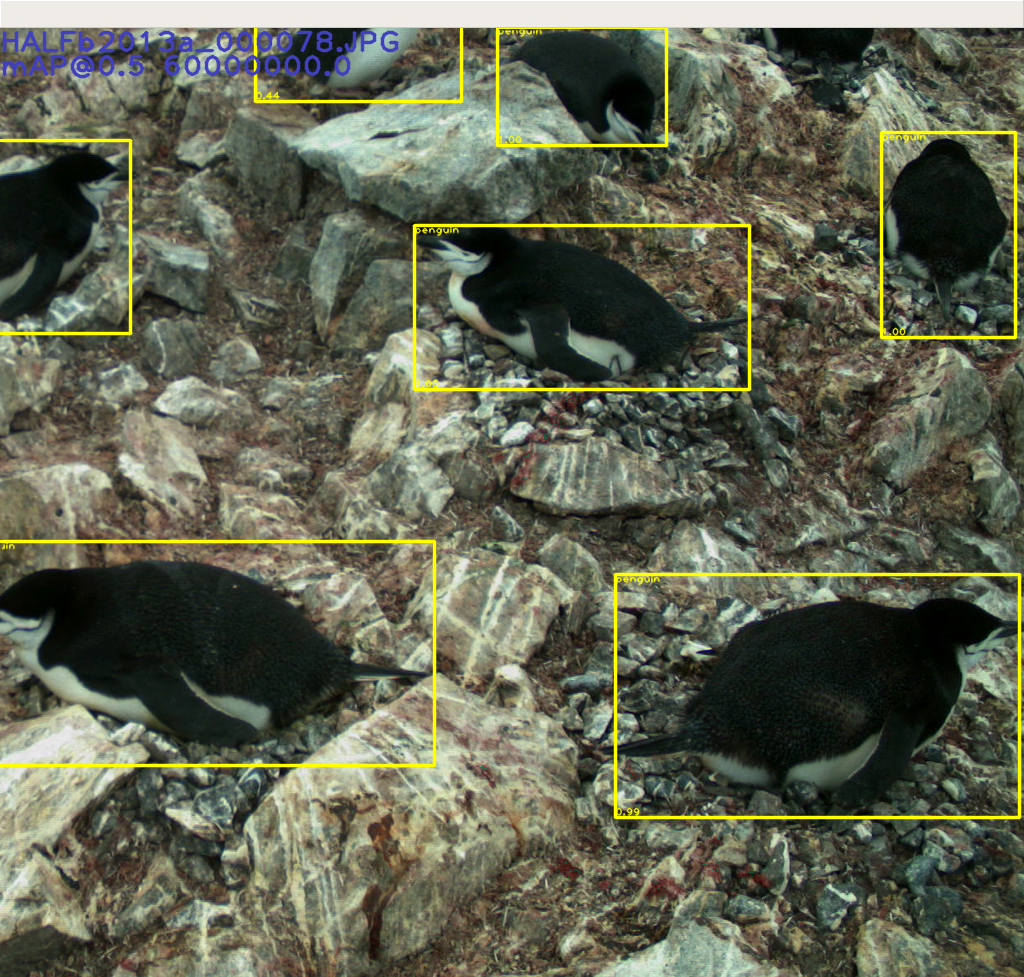
\includegraphics[width=0.95\linewidth]{figures/object/final.png}
  \caption{Final predictions after Non Maxima Suppression}
  \end{subfigure}%  
  \caption{Illustration of the stages of box prediction and refinement process}
  \label{fig:anchor_boxes}
\end{figure}


We use translation invariant anchor boxes as per \cite{Wang2017}, anchor boxes are the set of default locations and box sizes for which the \gls{CNN} can predict if and which object exists. It is unfeasible to provide a discrete set of boxes large enough to cover all possible object locations, therefore each anchor box is also modified by a scale and translation (details below in section \ref{sec:regression}) to fine tune anchor boxes to fit objects in the image.

Set of anchors boxes are used for each level with aspect ratios $ \in \{0.5, 1, 2\} $ and scales $ \in \{2^0, 2^{1/3}, 2^{2/3}\} $. For each feature map at level $k$, with a base scale of $ 2^{k + 2} $ pixels, the set of 9 anchor boxes (all combinations of aspect and scale) are tiled centred on each feature map pixel. 

In the case of counting, where circles are used for annotation only three anchor boxes are used, only the square aspect ratio is used at the same three scales. For all intents and purposes the circles with radius $r$ are treated as a square box with side lengths $2r$, and the box regression sub-network modified to produce only $3$ outputs (enforcing square aspect ratio for height and width).

Feature maps on levels $3$--$7$ are used for most datasets giving the smallest (square) anchor at $32\times32$ and the largest at $812\times812$. In the case of datasets with very small objects (for example, aerial penguin counting and wide angle counting of seals) we add in anchor boxes on level 2 which allow for objects as small as $16 \times 16$.

For those with smaller objects such as the aerial Adellie penguin counting, the tree branch detection and the seal counting an extra feature map is used giving anchor boxes as small as $16\times16$ and more densely tiled.

In training, anchor boxes are selected by matching on \gls{IOU} overlap with ground truth boxes. Each anchor is matched with the ground truth box with highest overlap. An anchor box matches a ground truth box as a positive if $ IoU >= 0.5 $, anchors with $ IoU < 0.4 $ are treated as negative, and those boxes with $ 0.5 > IoU >= 0.4 $ are ignored (omitted from either positive or negative for computing loss).

Ground truth boxes will match with potentially many anchor boxes, but those in close proximity and similar size may mean that boxes which would have otherwise matched do not, because anchors cannot be assigned to more than one ground truth.

\subsection{Total loss function}

The total loss function is defined as a balanced sum between box regression ($L_{loc}$) and class prediction loss ($L_{class}$). 

\begin{equation}
L  = L_{loc} + \lambda L_{class}
\label{eq:loss_total}
\end{equation}

\subsection {Box regression loss}
\label{sec:regression}


We use the anchor box encoding used in \gls{RCNN} \cite{Wang2017} for the purpose of calculating location loss. The loss is a smooth-L1 loss over regression target ($t^*_x, t^*_y, t^*_w, t^*_h \in t^*_i$) giving a transformation from an anchor box ($a_x, a_y, a_w, a_h$)  to a set of regression targets $t^*_i$ from the ground truth ($g_x, g_y, g_w, g_h$). 

The boxes are encoded as the offset of the centre in both directions (in proportion to the box size) and the log scale of height and width. The encoding of the four targets are given as:

\begin{equation}
\begin{split}
t^*_x = (g_x - a_x) a_w\\
t^*_y = (g_y - a_y) a_h\\
t^*_w = log(g_w / a_w)\\
t^*_h = log(g_h / a_h)\\
\end{split}
\label{eq:encoding_rcnn}
\end{equation}

The localisation loss can be directly computed from these targets and the output of the box prediction sub-network as the sum smooth-L1 regression of $t_i^* - t_i$. Smooth-L1 is a combination of L2 loss near the origin and L1 loss otherwise. It is given as:

\begin{equation}
L_{1;smooth} = 
\begin{cases*}
|x| & if $|x|>\alpha $ \\
\frac{1}{|\alpha|}x^2 & if $|x| \leq \alpha$
\end{cases*}
\label{eq:smooth_l1}
\end{equation}

The commonly used value $\alpha = 0.5$ is used here. The total localisation loss is then summed across matching (\gls{IOU} > 0.5) anchor truth boxes as:

\begin{equation}
L_{loc} = \sum_i{L_{1;smooth}(t_i^* - t_i)}
\label{eq:loss_loc}
\end{equation}

By rearranging the equations we can then do the reverse process and decode bounding boxes from box predictions $t_x, t_y, t_w, t_h$  and an anchor box. These predictions are then in units of pixels and given as the predictions of the object detection network (after a \gls{NMS} process to cull duplicates).

\begin{equation}
\begin{split}
p_x = a_x + t_x  a_w\\
p_y = a_y + t_y  a_h\\
p_w = exp(t_w) a_w \\
p_h = exp(t_h) a_h\\
\end{split}
\label{eq:decoding_rcnn}
\end{equation}

\subsection {Classification loss}
\label{sec:loss}

The experiments use a modified version of the Focal Loss \cite{Lin2017} to handle the class imbalance (negative vs. positive) present when sampling anchor box predictions densely.

Focal Loss \cite{Lin2017} re-weights the standard \gls{BCE} loss function to deal with a large number of easy negative examples in object detection (the number of unmatched anchor boxes greatly outnumbers the number of matched anchor boxes). Focal Loss enables dense sampling of negative examples present in an image. The standard approach in to dealing with the imbalance between positive and negative examples has been to sample the most significant negative examples to provide a certain positive to negative ratio.

As defined \cite{Lin2017}, we use the same terminology and variable naming for consistency. The basic two class \gls{CE} equation for binary prediction from the model classifier $p \in \left[0, 1\right]$, and label $y \in \{0, 1\}$  is given:

\begin{equation}
CE(p, y) = 
  \begin{cases*}
  -log(p) & if $y = 1$\\
  -log(1-p) & otherwise\\
  \end{cases*}
\label{eq:cross_entropy}
\end{equation}


The cross entropy can be rewritten by defining $p_t$ the prediction relative to the given label.

\begin{equation}
p_t = 
  \begin{cases*}
  p & if $y = 1$\\
  1 - p & otherwise\\
  \end{cases*}
\label{eq:class_prob}
\end{equation}

Allowing the \gls{CE} equation to be rewritten more simply:

\begin{equation}
CE(p_t) = -log(p_t)
\label{eq:short_cross_entropy}
\end{equation}


In order to deal with class imbalance the key idea of \cite{Lin2017} was to re-weight the classification loss to be smaller for well classified boxes (small $p_t$) and to be relatively much larger for badly classified boxes (large $p_t$). This was achieved by multiplying the cross entropy by a factor of $(1 - p_t)^\gamma $ with parameter $\gamma$ a sharpening parameter, to give the focal loss:

\begin{equation}
FL(p_t) = - (1 - p_t)^\gamma log(p_t)
\label{eq:focal_loss_p}
\end{equation}

Another way of dealing with class imbalance is to weight one of the classes (in the binary case given here either the positive c

A balanced cross entropy loss can then be written by adding a class weighting $\alpha \in \left[0, 1\right]$ the weight for the positive case in the two class setting, and an analogous $\alpha_t$:

\begin{equation}
\alpha_t = 
  \begin{cases*}
  \alpha & if $y = 1$\\
  1 - \alpha & otherwise\\
  \end{cases*}
\label{eq:balanced_weight}
\end{equation}

Then the balanced, focused, cross entropy is defined:

\begin{equation}
FL(p_t) = -\alpha_t (1 - p_t)^\gamma log(p_t)
\label{eq:focal_loss}
\end{equation}

I adopt the parameters given in \cite{Lin2017}, using $ \gamma = 2 $, and $ \alpha = 0.25 $. 

The total class loss is then given as the sum of the focal loss computed densely across all classes and anchor boxes in the image (except for anchor boxes between positive threshold and negative threshold $0.4 <= IoU < 0.5$ which are ignored). For $K$ classes, $p_i$ is the size $K$ prediction vector from the network for anchor box $i$ and $p^*_i$ is the size $K$ one hot target vector.

\begin{equation}
\begin{split}
L_{class} = \sum_i{\sum_{k \in K}FL(p_{ik}, p^*_{ik})}
\end{split}
\label{eq:class_loss}
\end{equation}

\subsection {Learning rate and Normalisation}

In \cite{Lin2017} a normalisation occurs over the total loss by the total number of positive matching anchor boxes, in order to average the error from the positive targets (making an assumption that the negative targets contribute a negligible amount to the total loss). As the datasets used in this work often don't contain any positive ground truth boxes it was necessary to avoid a division by zero. One method is to add a constant (representing the contribution of the negative classification targets) to the normalisation factor, the other is to divide by a constant value (essentially using a lower learning rate). I experimented a little with both options, finding either to be reasonably robust, the experiments in this work use a non normalised class classification loss.

In all experiments in this work (unless specified otherwise), the learning rate is set to $0.001$ and the balance factor $\lambda=2.5$. Total loss is averaged across each mini-batch, and batch sizes of $8$ are used.

\subsection{Inference and Non-maxima suppression}

In training a large set of anchor boxes are trained to classify each object detection (those overlapping each anchor box by $0.5$ or more). For the purposes of inference detecting more than one box for the same object is undesirable, so a greedy \gls{NMS} is used to eliminate multiple detections of the same object. Figure \ref{fig:anchor_boxes} shows the effect of applying a \gls{NMS} on box predictions, (b) shows the regressed predictions where many boxes overlap the same object (c) shows the result of the \gls{NMS}, leaving a single box on each object. In this work a standard \gls{NMS} procedure as per \cite{Wang2017} is used, where boxes are selected from most-confident to least-confident, boxes overlapping lower confidence boxes by more than an \gls{IOU} threshold (in this work $0.5$) are eliminated.

The use of \gls{NMS} has presents some problems in object detectors notably the inability to handle highly overlapping objects well. Objects high overlap by more than $0.5$ are impossible to accurately detect for such a detector. When used for annotating crowded objects the inability of the object detector to accurately predict highly overlapping objects means in some datasets the user spends a lot of time correcting artefacts caused by limitation of the object detector (by no means limited to \gls{NMS}).


\section{Evaluation metrics}
\label{sec:evaluation_metrics}

The most common metric used in object detection is that of \gls{AP}, as popularised by the Pascal VOC challenge \cite{Everingham2008} and later the COCO dataset \cite{Lin2014}. The \gls{AP} is essentially the area under a recall-precision graph for a particular matching threshold and varies from $0$  to $1$. it's major attraction is that it avoids the need for a detection threshold. It provides a single relatively easy to understand metric which measures precision, recall as well as localisation accuracy (for a particular threshold).

Matches are found by a greedy algorithm in each image (similar to that used in \gls{NMS} above) where the predictions are matched against ground truth boxes from a most-confident to lead-confident order. Each prediction matches it's highest overlap ground truth box where the overlap exceeds the \gls{IOU} threshold (amongst ground truth boxes already unmatched). Matches from all images are then merged and sorted by confidence level of the prediction of the match. True-positives ($tp$) and false-positives ($fp$) are found by counting matched and unmatched predictions from high-to-low confidence, false-negatives ($fn$) are determined at each point by subtracting true-positives from the total ground truth count. 

\begin{equation*}
\begin{split}
p_i = \frac{tp_i}{fp_i + tp_i}\\
r_i = \frac{tp_i}{tp_i + fn_i}
\end{split}
\end{equation*}

From there recall ($r$), and precision ($p$) levels can be determined at the confidence level of each prediction. Special cases are added for $r_0=0, p_0=1$ and $p_n=1, r_n=0$, the precision levels are then made monotonic decreasing:

\begin{equation}
\hat{p_i} = \max_{j \in [i..n]}{p_j}
\end{equation}

\gls{AP} can then be calculated by using trapezoid summation:

\begin{equation}
AP = \sum_{i \in [0..n-1]}\frac{\hat{p_i} + \hat{p}_{i + 1}}{2}
\end{equation}



\gls{mAP} is then defined as the mean of \gls{AP} over classes, and is often notated $mAP@IoU$ for a particular matching threshold IoU, for example $mAP@0.5$ is metric used for evaluation for the Pascal VOC \cite{Everingham2008}, but $mAP@0.75$ for example provides a much stricter matching criteria on the allowable localisation error. In this work we are much more interested in the stricter matching criteria, because a match overlap of $0.5$ represents a box which the annotator will need to manually correct.

To produce a single metric taking into account localisation accuracy \cite{Lin2014} defined a metric COCO \gls{AP} as the mean of \gls{mAP} at a series of matching thresholds $ IoU \in [0.5 : 0.05 : 0.95] $, confusingly this mean-\gls{mAP} is termed just \gls{AP}. We follow this convention however, where we use \gls{mAP} and refer to \gls{AP} as the COCO \gls{AP}.

There are downsides to the \gls{mAP} metric. The precision-recall graph created using decreasing confidence considers only the order of detection confidence. This has implications that the level of false positives which occur at lower confidence than the last true-positive are ignored, in addition the margin between confidence levels is ignored, so the sensitivity to change in confidence levels is not taken into account. The threshold on \gls{IOU} overlap also means that all true-positives which meet the localisation threshold are treated equally, matches which match the ground truth perfectly are scored the same as those which meet only the minimum match threshold. Alternatives exist, although arguably not as easy to understand as \gls{mAP}, for example \cite{Oksuz2018} which tries to weight true-positives for localisation accuracy, as well as attempting to provide a way to determine the ideal detection threshold.



\section {Learning schedule}
\label{sec:schedule}

\begin{figure}[h]
  \centering
  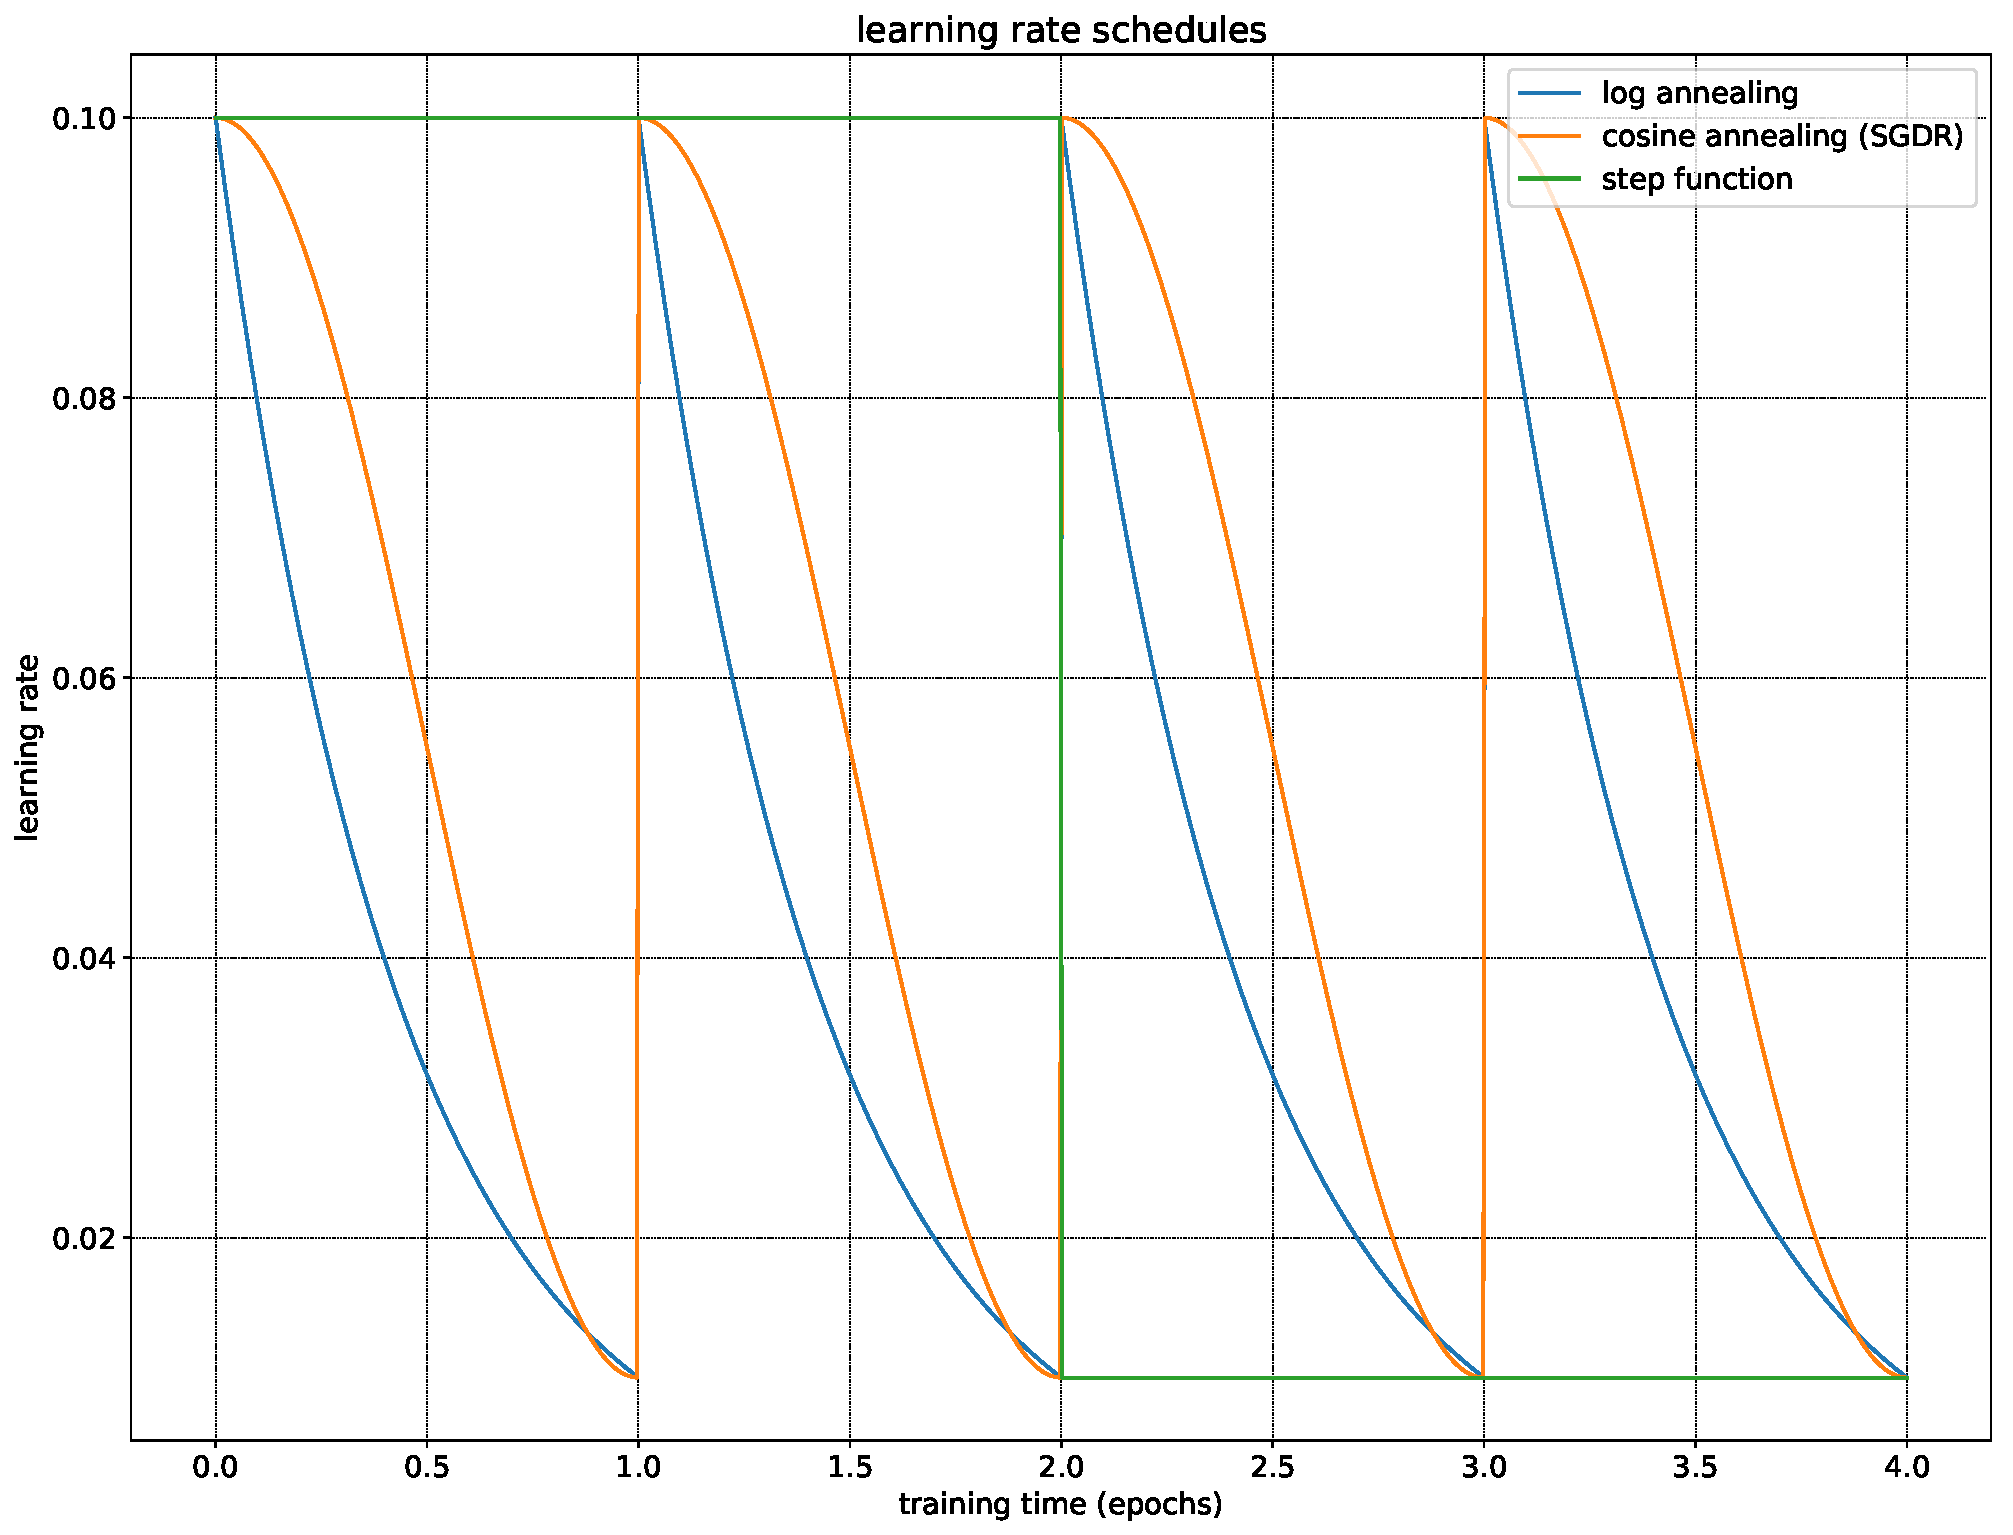
\includegraphics[width=1.0\linewidth]{charts/training/lr_schedules.pdf}
  \caption{Comparison of learning rate schedules, cyclical learning rates and traditional step function.  }  
  \label{fig:lr_schedule}
\end{figure}

In order to facilitate continuous online learning where examples are added over the training lifetime, a cyclical learning rate is used and relatively short learning epochs are used. Epochs are set at a fixed size ($1024$ unless otherwise specified), using a uniform random sampling. Learning rates are set for each batch, reducing over an epoch by a factor of $10$, using a logarithmic annealing shown in equation \ref{eq:log_annealing}. Where $base$ is the base learning rate, and $ t \in [0, 1) $ is the progress across an epoch.

\begin{equation}
log_annealing(t) = exp(ln (lr_min) (1 - t) + ln(lr_max)  t)
\label{eq:log_annealing}
\end{equation}

For comparison the learning rate schedule used in \gls{SGDR} \cite{Loshchilov2016}, which has more weight on the highest and lowest learning rates, but otherwise similar.

\begin{equation}
cosine_annealing(t) = lr_min +  1/2 (lr_max - lr_min) (1 + cos (t \pi)
\label{eq:cosine_annealing}
\end{equation}

A comparison of the cyclical learning rates compared to a standard learning rate step schedule is shown for an $8$ epoch training schedule in figure \ref{fig:lr_schedule}.



\section{Methods of inference for high resolution images}
\label{sec:highres_inference}

\begin{figure}[h]
  \centering
  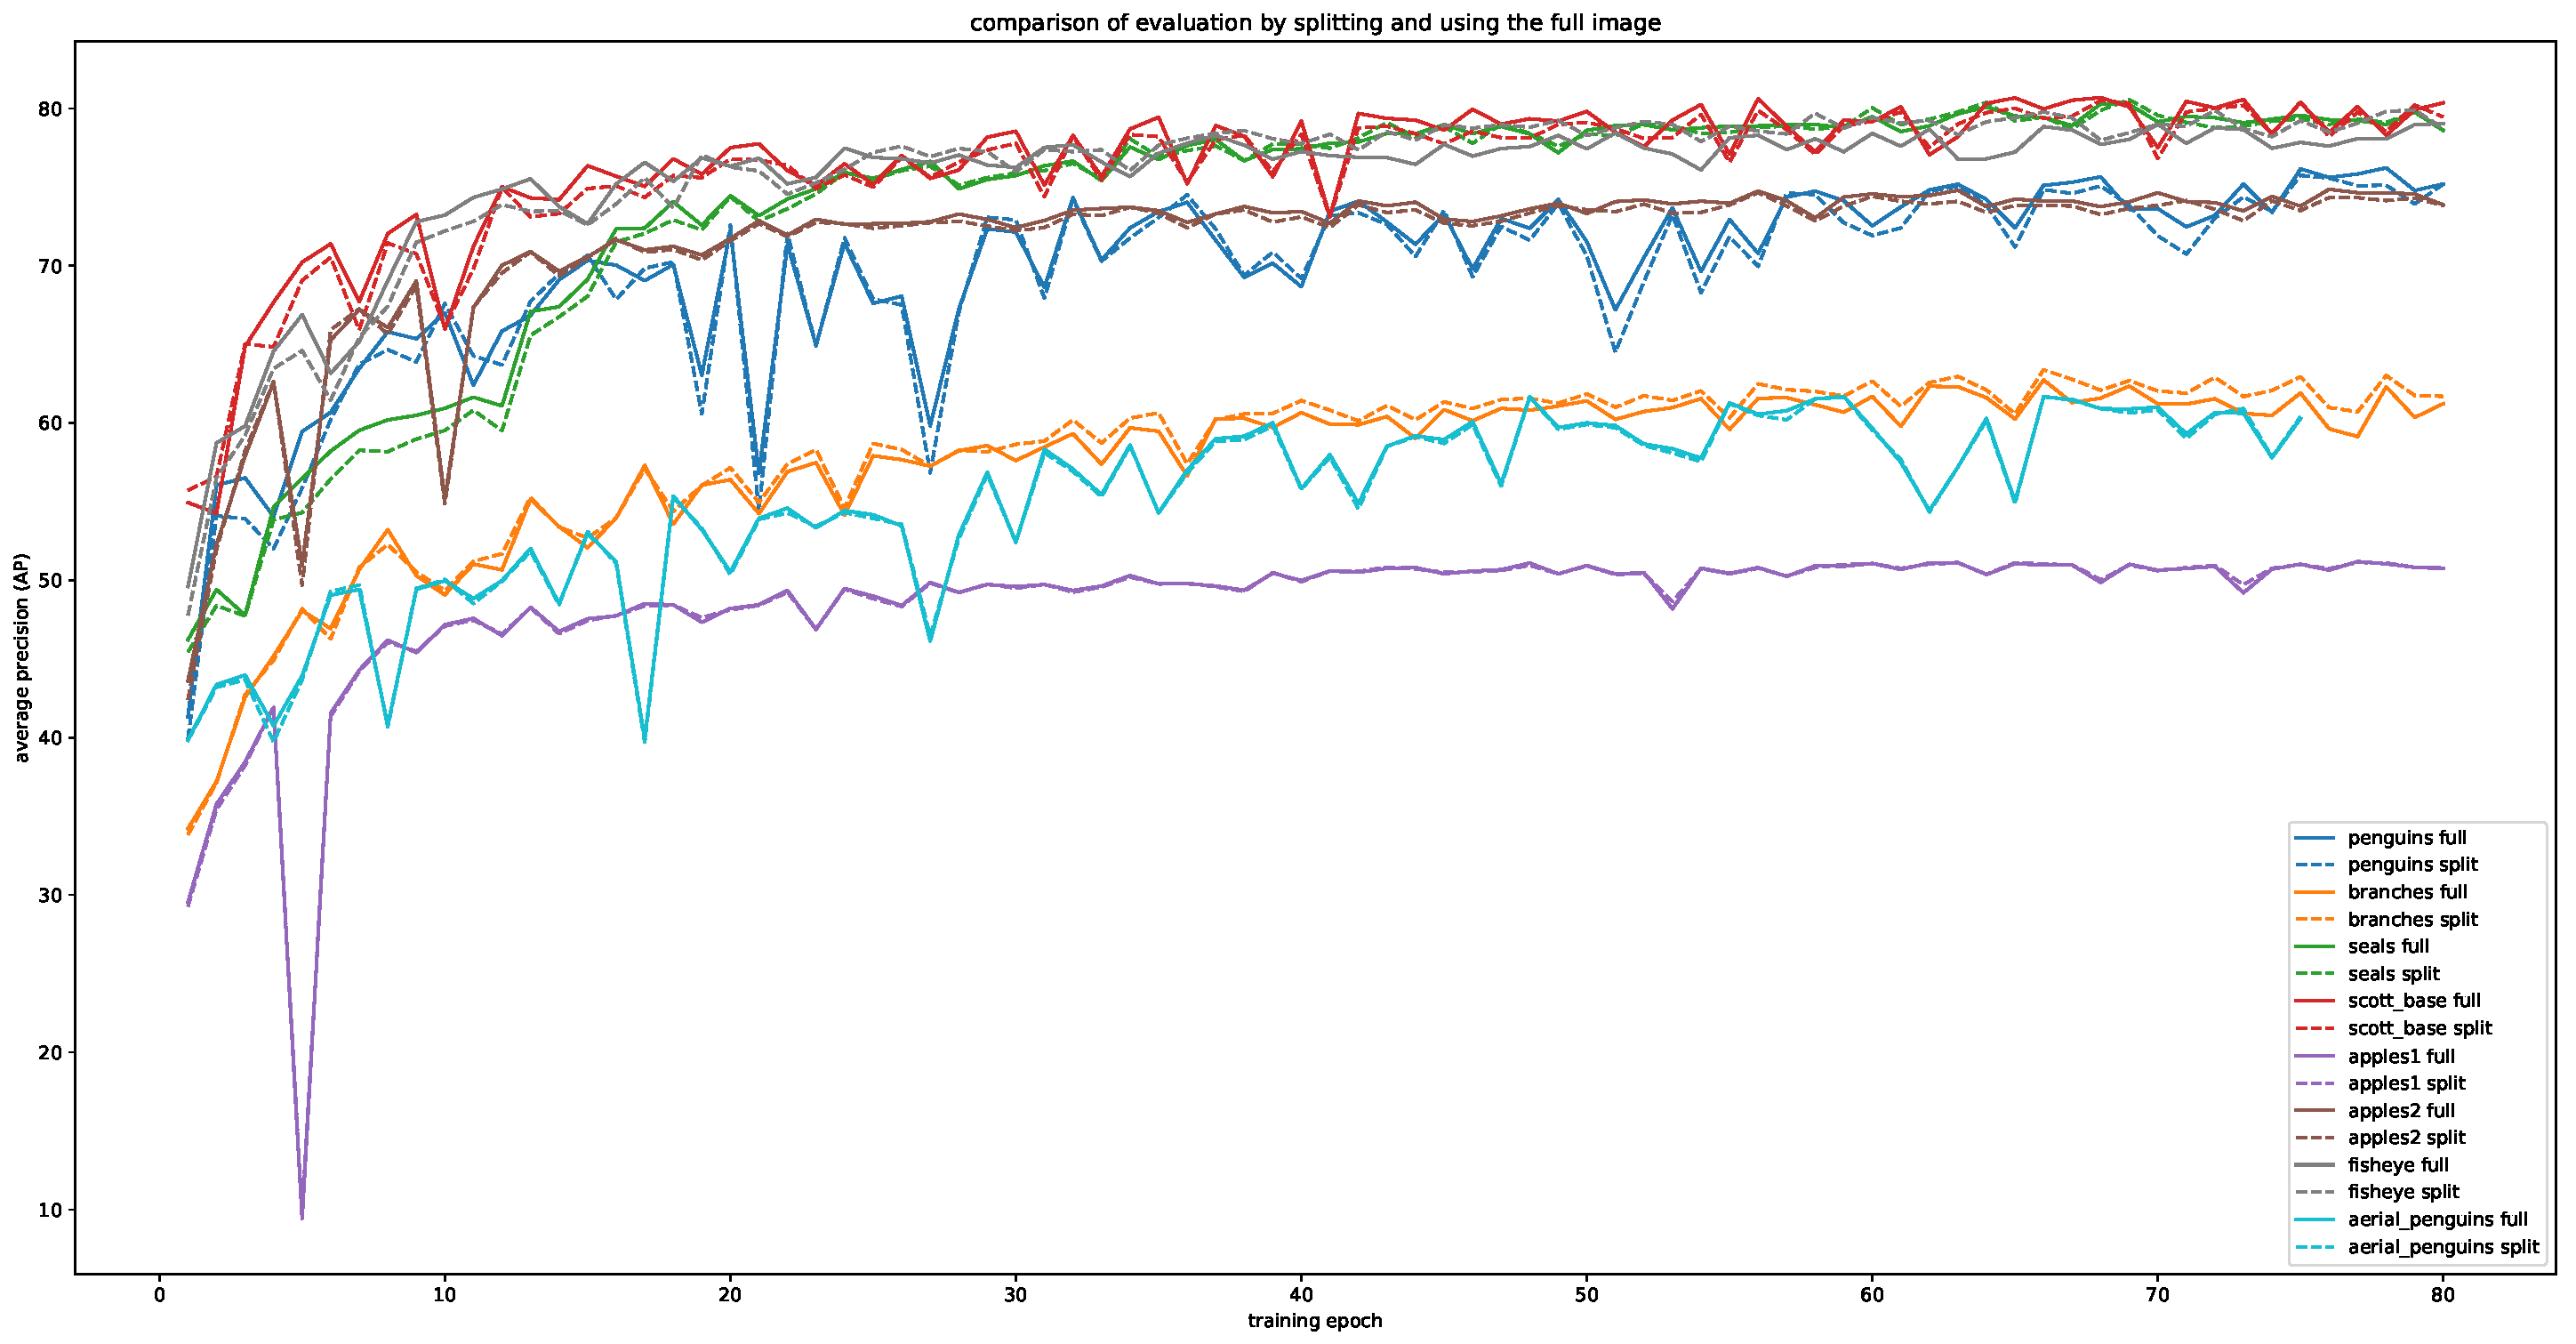
\includegraphics[width=1.0\linewidth]{charts/training/splits.pdf}
  \caption{Comparison of different inference methods, training on crops and evaluating on full images. The dashed lines combine multiple inferences using tiling, and the solid lines are inference using the full image.  }  
  \label{fig:inference_method}
\end{figure}

I look at two different possibilities for performing inference on a full resolution image using an object detector network trained only on crops of images; (a) pass in the full image using the property that the network is 'Fully Convolutional', (b) tile images the same size as training crops and collapse the predictions using a combined \gls{NMS}. In order to facilitate this idea the box annotations on the edge of images are estimates of the full bounds of the object; and the anchor boxes are not cropped to the edge of the image.

Object detection networks are flexible and work across a range of input image resolutions. All layers are either convolutions or do not reshape the feature maps (aside from up/down sampling). As a result, passing in a larger image results in a larger output sets at each layer of the pyramid. For an object detection network this corresponds to a larger set of anchor boxes (given that the anchor boxes are translation invariant). The concern is that the up/down sampling behaviour is slightly different for input sizes depending if they're odd or even relative to powers of two. I found this is a legitimate concern, though largely negated if the training crop size is a power of two or a multiple of a power of two.

The second inference method is to tile multiple 'raw' inferences across the full image size using a certain overlap buffer region, the result is sets of overlapping predictions. These overlapping predictions can be decimated using a combined \gls{NMS}, such that it removes duplicates overlapping from two neighbouring tiles. The concern with this method is that edge detections are possibly inaccurate and may produce erroneous predictions which are not removed by \gls{NMS} because of their inaccurate localisation. 

Both methods are tested by testing against the validation set of several different training runs. It can be seen in figure-\ref{fig:inference_method} that both perform very similarly. If there is ever a difference; sometimes one is marginally better, sometimes the other is marginally better, even within the same training run.

\section {Effect of scale and crop size}
\label{sec:scale_crop}

High resolution images present a cost in terms of training (and inference) time, also in terms of memory and data required to transfer over a network. I expect the trade-off to be be worthwhile however. High resolution images are undoubtedly easier to annotate, small details become clear and using down scaled images often makes even the annotation task ambiguous. It is not necessary to feed the model images of the same resolution as the user annotates, but if a human annotator has trouble with ambiguity it seems a reasonable assumption that a \gls{CNN} will also struggle.

Especially for datasets with many small examples, the datasets used here (see chapter for details \ref{chap:7}) contain many small objects, and many objects with a high degree of uncertainty and ambiguity.



The full resolution images do provide the best accuracy, although in many of the datasets half resolution provided almost the same accuracy while providing much faster training and inference. At half resolution an ensemble could be trained in similar time to training one network at full resolution and used to provide uncertainty measurements. On the other hand, as seen below in section-\ref{sec:lr_schedule_exp} the training accuracy is limited by the size of the dataset more than the training time, which is severely dependent on human annotation time which will allow plenty of time for training at high resolution.

Using a larger crop size proved better in three of the four datasets, however for apples it trained faster and achieved roughly the same level of accuracy as the larger crop. Crop size could perhaps be adjusted automatically based on the largest size of the objects.


\section {Learning rate scheduling}
\label{sec:lr_schedule_exp}

I expect cyclical learning rates to much better cope with a stream of new examples provided incrementally, this is important if the model is to provide good assistance to an annotator in a timely fashion. 


\subsection {Single vs. multi-class training}
\label{sec:lr_schedule_exp}

In this experiment I examine the idea that for the purposes of providing annotation assistance, that it is better to focus on a single class, or few classes (from the point of view of training an object detector to aid further annotation). 

\subsection{Single or few-class vs. multi-class}

Given the the experiment in section-\ref{sec:lr_schedule_exp} it is seen that the accuracy of the object detector correlates with the number of examples

With appropriate preparation, annotating a single class at a time should enable a larger number of examples of that class in a shorter period. This is highly dependent on the dataset and the preparation before annotation begins. Some level of pre-sorting or image selection becomes crucial if classes are very sparsely distributed in the input images; for example if there are a lot of classes, but only a hand-full in any particular image.

The datasets used in this work are either single or few-class, with multiple instances per image; with the exception of the \emph{scallops} dataset, where despite being a single class annotation the instances are sparsely distributed amongst the images.







\section{Other factors}

Here I discuss some other factors which had large impact on the performance of the object detection network, but have not been quantified.

\begin{itemize}
    \item {\bf Larger and more sophisticated models}
Primarily we used ResNet-18 \cite{He2015} as the backbone network in all the experiments, there are many larger more sophisticated networks, of the networks used to classify ImageNet ResNet-16 is one of the simplest. Other networks work at least equally as well, but I did not find significant improvement at the expense of slower training and evaluation.
    \item {\bf Shared weights in class prediction sub-network}
RetinaNet \cite{Lin2017} used shared weights for it's class prediction sub-network (figure \ref{fig:prediction_subnet}) at different resolution outputs (but not between box localisation sub-networks). I found in the small scale datasets used in this work that shared weights on the class sub-network significantly slows initial learning. Extra residual layers in the decoder side of the network (figure \ref{fig:decoder_block}) improved this significantly, but not entirely.
    \item {\bf Initialisation matters}
Using the initialisation in \cite{Lin2017} where all new convolutions added to the backbone are initialised with $\sigma=0.1$ (and no bias). The final layer of the classification sub-network has bias initialised to $b = −log((1 − \pi)/\pi) $ whereby at the start of training every anchor box is assigned confidence of $~\pi$, we use $\pi=0.01$. With this initialisation the network becomes robust to a wide range of resolutions and learning rates.

\end{itemize}

\section {Conclusion}

This chapter described the object detector used behind the annotation tool, parameters used, methods of training and described some of the rationale for the differences with published literature. Chapter-\label{chap:annotation} attempts to evaluate the annotation software as a whole through it's practical use in annotating several datasets. Some of those datasets annotated this way I have then used to evaluate some of the assumptions used in the design, and the parameter set used in this chapter. 


